\documentclass[english]{short-notes}

\usepackage{math-ag}

\addbibresource{global.bib}
%\bibliography{global.bib}

\title{Perverse coherent sheaves}
\subtitle{Notes for oral exam}
\author{Clemens Koppensteiner}

\newcommand\derived{\mathbf D}
\newcommand\derivedcoh{\derived_{\mathrm{coh}}}
%\renewcommand\cat{\mathscr}
\let\setset\cover
\newcommand\inv{\mathrm{inv}}
\newcommand\alg{\mathrm{alg}}

\begin{document}

\renewcommand\top{\mathrm{top}}
\renewcommand\dual{\mathbb D}

\maketitle

\tableofcontents

\section{Introduction}

In the following $X$ will always be complex variety and $G$ an affine complex group variety.
We assume that $X$ has a dualizing complex (see Section \ref{sec:dualizing_complex}) that is $G$-equivariant (Section \ref{sec:equivariance}).
This is not the most general setting, but should suffice for this introduction.

The presentation of perverse coherent sheaves is based upon \cite{Bezrukavnikov:arXiv:PerverseCoherentSheaves,ArinkinBezrukavnikov:arXiv:PerverseCoherentSheaves}.
We will use the language of equivariant sheaves (i.e.~\cite{Bezrukavnikov:arXiv:PerverseCoherentSheaves}), rather that stacks.

\section{Preliminaries}

\subsection{Category theory}

\subsubsection{Derived categories}\label{sec:derived_categories}

E.g., \cite{Verdier:1977:CategoriesDerivees}, \cite[Chapter~III]{GelfandManin:2003:MethodsOfHomologicalAlgebra} and \cite[Chapter 1]{Hartshorne:1966:ResiduesAndDuality}.

\subsubsection{Triangulated categories}\label{sec:triangulated_categories}

References are \cite{Verdier:1977:CategoriesDerivees}, \cite[Chapter IV]{GelfandManin:2003:MethodsOfHomologicalAlgebra} and \cite[Section 1.1]{BeilinsonBernsteinDeligne:1982:FaisceauxPervers}.

\begin{Def}
    A \emph{triangulated category} consists of an additive category $\cat D$ together with
    \begin{itemize}
        \item an automorphism (or auto-equivalence) $T\colon \cat D → \cat D$, called the \emph{translation functor}, and
        \item a collection of sequences
            \[ X \xrightarrow{u} Y \xrightarrow{v} Z \xrightarrow{w} TX, \]
            called \emph{distinguished} triangles,
    \end{itemize}
    satisfying the following axioms, where we write $X[1] \coloneq TX$,
        \begin{enumerate}
            \item[(TR~1)]
                Any triangle (i.e.\ sequence $X → Y → Z → X[1]$) isomorphic to a distinguished triangle is distinguished.
                Every morphism $u\colon X → Y$ is contained in a distinguished triangle $X \xrightarrow{u} Y → Z → X[1]$.
                Every triangle of the form $X \xrightarrow{\id} X → 0 → X[1]$ is distinguished.
            \item[(TR~2; rotation)]
                A triangle $X \xrightarrow{u} Y \xrightarrow{v} Z \xrightarrow{w} X[1]$ is distinguished, if and only if $Y \xrightarrow{v} Z \xrightarrow{w} X[1] \xrightarrow{-u[1]} Y[1]$ is distinguished.
            \item[(TR~3; morphisms)] 
                If $X \xrightarrow{u} Y \xrightarrow{v} Z \xrightarrow{w} X[1]$ and
                $X' \xrightarrow{u'} Y' \xrightarrow{v'} Z' \xrightarrow{w'} X'[1]$
                are distinguished, then for each morphism $(f,g)\colon u → u'$ there exists a morphism $h\colon Z → Z'$ such that $(f,g,h)$ is a morphism of triangles (where a morphism of triangles is defined as the obvious commutative diagram).
            \item[(TR~4; octahedral axiom)]
                \remark{%
                    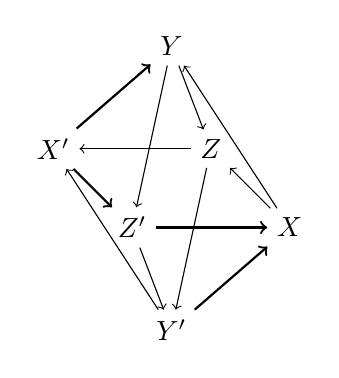
\begin{tikzpicture}[x={(1cm,0)}, y={(0.5cm,-0.5cm)}, z={(0,1.8cm)},baseline={(0,1)}]
                        \node (Y) at (0,0,1) {$Y$};
                        \node (X) at (1,1,0) {$X$};
                        \node (Z) at (1,-1,0) {$Z$};
                        \node (X') at (-1,-1,0) {$X'$};
                        \node (Z') at (-1,1,0) {$Z'$};
                        \node (Y') at (0,0,-1) {$Y'$};

                        \path[->]
                            (X) edge (Z) edge (Y)
                            (Z) edge (X') edge (Y')
                            (X') edge[thick] (Y) edge[thick] (Z')
                            (Z') edge[thick] (X) edge (Y')
                            (Y) edge (Z) edge (Z')
                            (Y') edge[thick] (X) edge (X');
                    \end{tikzpicture}%
                }
                If $X \xrightarrow{u} Y \xrightarrow{i} Z' → X[1]$,
                $Y \xrightarrow{v} Z \xrightarrow{} X' \xrightarrow{j} Y[1]$, and
                $X \xrightarrow{w} Z \xrightarrow{} Y' \xrightarrow{} X[1]$
                are distinguished triangles such that $w = v∘u$, then there exist morphisms $f\colon Z' → Y'$ and $g\colon Y' → X'$ such that
                \begin{enumerate}[1)]
                    \item $(\id[X],v,f)$ is a morphism of triangles;
                    \item $(u, \id[Z],g)$ is a morphism of triangles;
                    \item $Z' \xrightarrow{f} Y' \xrightarrow{g} X' \xrightarrow{i[1]∘j} Z'[1]$ is a distinguished triangle.
                \end{enumerate}
    \end{enumerate}
    A \emph{functor of triangulated categories} is a functor of the underlying categories which commutes with the translation functors and sends distinguished triangles to distinguished triangles.
\end{Def}

\begin{Ex}
    Let $\cat A$ be an additive category and $\mathbf K\cat A$ the category of complexes of objects of $\cat A$ and $\Hom_{\mathbf K\cat A}(K,L)$ the set of homotopy classes of morphisms of complexes from $K$ to $L$.
    Let $TK = K[1]$ be defined by $(K[1])^n = K^{n+1}$ (with a sign change in the differential).
    In $\mathbf K\cat A$ the distinguished triangles are gives by $K \xrightarrow{u} L → \operatorname{cone}(u) → K[1]$, giving $\mathbf K\cat A$ the structure of a triangulated category.
    Here we need to work in the homotopy category of complexes, as otherwise the triangle $K \xrightarrow{\id} K → 0 → K[1]$ wouldn't be distinguished (the mapping cone of $\id$ is only homotopic to 0).
    Also note that if $u\colon K → L$ is injective, then $\operatorname{cone}(u) \cong L/K$, so that every short exact sequence of complexes is a distinguished triangle.

    If $\cat A$ is Abelian, this structure descends to the derived category $\derived \cat A$.
\end{Ex}

\begin{Def}
    Let $\cat D$ be a triangulated category and $\cat A$ an Abelian category.
    A functor $F\colon \cat D → \cat A$ is called \emph{cohomological} if it maps each distinguished triangle $X → Y → Z → X[1]$ to an exact sequence $F(X) → F(Y) → F(Z)$.
\end{Def}

\begin{Ex}
    For any $X ∈ \cat D$ the functors $\Hom_{\cat D}(X,\cdot)$ and $\Hom_{\cat D}(\cdot, X)$  are cohomological (the second one being defined on the opposite triangulated category (with translation functor the inverse of $T$ and reading distinguished triangles the other way)).
    Hence, if $F\colon \cat D → \cat A$ is cohomological, it induces a long exact sequence
    \[
    \dotsc → FX → FY → FZ → FTX → FTY → \dotsc
    \]
    for each distinguished triangle $X → Y → Z → X[1]$ (using TR~2 repeatedly).
\end{Ex}

\subsubsection{t-categories}\label{sec:t-categories}

References are \cite[Section 1.3]{BeilinsonBernsteinDeligne:1982:FaisceauxPervers} and \cite[Section IV.4]{GelfandManin:2003:MethodsOfHomologicalAlgebra}.

\begin{Def}
    A \emph{t-category} is a triangulated category $\cat D$ together with a pair $(\cat D^{≤0},\cat D^{≥0})$ of full subcategories, called a \emph{t-structure}, such that, writing $\cat D^{≤n} = \cat D^{≤0}[n]$ and $\cat D^{≥n} = \cat D^{≥0}[n]$, the following conditions hold:
    \begin{enumerate}
        \item if $X ∈ \cat D^{≤0}$ and $Y ∈ \cat D^{≥1}$, then $\Hom_{\cat D}(X,Y) = 0$;
        \item $\cat D^{≤0} ⊆ \cat D^{≤1}$ and $\cat D^{≥0} ⊇ \cat D^{≥1}$;
        \item for each $X ∈ \cat D$ there exists a distinguished triangle $A → X → B → A[1]$ such that $A ∈ \cat D^{≤0}$ and $B ∈ \cat D^{≥1}$.
    \end{enumerate}

    The full subcategory $\cat D^{≤0} ∩ \cat D^{≥0}$ is called the \emph{heart} or \emph{core} of the t-structure, sometimes denoted $\cat D^\heartsuit$.
\end{Def}

\begin{Ex}
    If $\cat A$ is an Abelian category, then its derived category $\derived \cat A$ admits a standard t-structure given by
    \begin{align*}
        \derived \cat A^{≤0} &= \{ F ∈ \derived\cat A : H^j(F) = 0 \text{ for all } j > 0 \}, \\
        \derived \cat A^{≥0} &= \{ F ∈ \derived\cat A : H^j(F) = 0 \text{ for all } j < 0 \}.
        \qedhere
    \end{align*}
\end{Ex}

\begin{Prop}
    The inclusions $\cat D^{≤n} → \cat D$ (resp.~$\cat D^{≥n} → \cat D$) admit right (resp.~left) adjoint functors $τ^{≤n}\colon \cat D → \cat D^{≤n}$ (resp.\ $τ^{≥n}\colon \cat D → \cat D^{≥n}$), called the \emph{truncation functors}.
\end{Prop}

These functors $τ^{≤0}$ and $τ^{≥1}$ are given by the third property of the definition of a t-structure. 
The other truncation functors are just translates.

\begin{Ex}
    For the standard t-structure of a derived category the truncation functors are the usual (non-naive) truncation functors.
\end{Ex}

The main result about t-structures in the following theorem that provides a convenient way to identify Abelian subcategories.

\begin{Thm}
    The heart of a t-category is an Abelian category that is stable under extensions (i.e.\ for every distinguished triangle $X → Y → Z → X[1]$ with $X$ and $Z$ in the heart, $Y$ is also in the heart).
\end{Thm}

\begin{Prop}
    The functor $H^0 = τ^{≤0} ∘ τ^{≥0} \cong τ^{≥0} ∘ τ^{≤0}\colon \cat D → \cat D^{\heartsuit}$ is a cohomological functor.
\end{Prop}

We set $H^n = H^0 ∘ [n]$.

\begin{Def}
    Let $F\colon \cat{D₁} → \cat{D₂}$ be a functor of triangulated categories.
    We say that $F$ is \emph{left t-exact} (resp.\ \emph{right t-exact}) if $F(\cat{D₁}^{≥0}) ⊆ \cat{D₂}^{≥0}$ (resp.\ $F(\cat{D₁}^{≤0}) ⊆ \cat{D₂}^{≤0}$).
    It is \emph{t-exact} if it is both left and right t-exact.
\end{Def}

\begin{Prop}
    Let $i\colon \cat{D₁}^\heartsuit → \cat{D₁}$ be the inclusion.
    If $F\colon \cat{D₁} → \cat{D₂}$ is left/right t-exact, then $H^0 ∘ F ∘ i\colon \cat{D₁}^\heartsuit → \cat{D₂}^\heartsuit$ is a left/right exact functor of Abelian categories.
\end{Prop}


\subsection{Operations on sheaves}

For any morphism $f\colon X → Y$ of ringed spaces, $\sheaf F$ a sheaf of $\O_X$-modules and $\sheaf G$ a sheaf of $\O_Y$-modules, recall the definitions of the functors mentioned above:
\begin{itemize}
    \item $f_*\sheaf F(V) = \sheaf F(f^{-1}V)$, made into an $\O_Y$-module via the given map $\O_Y → f_*\O_X$.
    \item $f^{-1}\sheaf G(U) = \varprojlim_{V ⊇ U} \sheaf G(U)$, is not an $\O_X$-module.
    \item $f^*\sheaf G = f^{-1}\sheaf G \otimes_{f^{-1}\O_Y} \O_X$.
    \item $f_!\sheaf F(V) = \{ s ∈ F(f^{-1}V) : \res{f}{\supp s}\colon \supp s → U\text{ is proper}\}$, in particular if $f$ is proper (e.g.\ a closed immersion), then $f_! = f_*$.
        If $j\colon U → X$ is an open inclusion, then $j_!\sheaf F(V)$ is the sheafification of the presheaf $\sheaf H(V) = \sheaf F(V)$ if $V ⊆ U$ and $\sheaf H(V) = 0$ otherwise.
    \item If $f\colon X → Y$ is an immersion of locally closed subspace, then $f^!\sheaf G = f^*\sheaf H$, where $\sheaf H(U) = \{ s ∈ G(U) : \supp s ⊆ X\}$.
        In particular, if $f$ is an open immersion, then $f^! = f^*$.
        In general one defines $Rf^!$ as the right adjoint to $Rf_!$ on the derived category.
\end{itemize}

Let $j\colon U \hookrightarrow X$ be an open subvariety and $i\colon X\setminus U \hookrightarrow X$ the complement.
Then there are two sequences of adjoint functors $(j_!, j^! = j^*, j_*)$ and $(i^*, i_* = i_!, i^!)$.
The adjunctions give a distinguished triangles (in $\derived^+(\catModules{\O_X})$)
\[
j_!j^*\sheaf F → \sheaf F → i_*i^* \sheaf F
\quad\text{and}\quad
i_*i^!\sheaf F → \sheaf F → j_*j^* \sheaf F.
\]

\subsection{Perverse constructible sheaves}

Perverse sheaves were introduced in \cite{BeilinsonBernsteinDeligne:1982:FaisceauxPervers}.
References include \cite[Chapter~8]{HottaTakeuchiTanisaki:2008:DModulesPerverseSheavesRepresentationTheory} and \cite[Chapter~13]{PetersSteenbrink:2008:MixedHodgeStructures}.

Let $\setset S$ a finite stratification of $X$ with each stratum locally closed, smooth and equidimensional.
Further we assume that the closure of each stratum is a union of strata.

Let $\derived_{c-\setset S}(X)$ be the full subcategory of $\derived(\catModules{ℂ_X})$ consisting of objects with constructible cohomology with respect to $\setset S$ (a sheaf is constructible with respect to $\setset S$ if the restrictions to each stratum is a locally constant sheaf of $ℂ$-modules).

\begin{Def}[{\cite[Définition~2.1.2]{BeilinsonBernsteinDeligne:1982:FaisceauxPervers}}]
    A function $p\colon ℕ → ℤ$ is called a \emph{perversity}.
    For $S ∈ \setset S$ set $p(S) = p(\dim_{\top} S) = p(2\dim_{\alg} S)$.
    Define the following full subcategories of $\derived_{c-\setset S}(X)$:
    \begin{align*}
        \perv\derived^{≤0}_{\setset S}(X) & = \{ K ∈ \derived_{c-\setset S}(X)(X,) : H^ni_S^*K = 0 \text{ for each } S ∈ \setset S \text{ and } n > p(S) \}, \\
        \perv\derived^{≥0}_{\setset S}(X) & = \{ K ∈ \derived^+_{c-\setset S}(X)(X) : H^ni_S^!K = 0 \text{ for each } S ∈ \setset S \text{ and } n < p(S) \},
    \end{align*}
    where $i_S \colon S \hookrightarrow X$ is the inclusion.
\end{Def}

\begin{Thm}
    $(\perv\derived^{≤0}_{\setset S}(X),  \perv\derived^{≥0}_{\setset S}(X))$ is a t-structure on $\derived_{c-\setset S}(X)$ and induces one on $\derived^*_{\setset S}(X)$ for $*={+},{-},{b}$.
\end{Thm}

The objects in the heart of this t-structure are called \emph{perverse sheaves} with respect to $\setset S$.

One can make this definition independent of the stratification by taking a limit over all stratifications.
Explicitly this leads to the following definition:

\begin{Def}
    Let $p\colon ℕ → ℤ$ be a perversity function.

    Let $\perv\derived^{≤0}(X)$ be the full subcategory of $\derived_c^b(X)$ consisting of objects $F$ for which $H^n(i_S^*F) = 0$ for every locally closed subvariety $S$ and any $n > p(S)$. 

    Let $\perv\derived^{≥0}(X)$ be the full subcategory of $\derived_c^b(X)$ consisting of objects $F$ for which $H^n(i_S^!F) = 0$ for every locally closed subvariety $S$ and any $n < p(S)$.
\end{Def}

This isn't the shortest possible definition, but the one that most easily generalizes to the coherent setting.

\begin{Thm}
    If the perversity function $p$ and the dual perversity $\bar p(n) = -n - p(n)$ are both decreasing, then  $(\perv\derived^{≤0}(X),  \perv\derived^{≥0}(X))$ is a t-structure on $\derived_{c}^b(X)$.
\end{Thm}

\subsection{Equivariant sheaves}\label{sec:equivariance}

Let $a\colon G×X → X$ be the action and $p\colon G×X → X$ the projection.

\begin{Def}
    A \emph{$G$-equivariant coherent sheaf on $X$} is a pair $(\sheaf F, φ)$ consisting of a coherent sheaf $\sheaf F$ on $X$ and an isomorphism $α^*\sheaf F \isoto p^*\sheaf F$.
\end{Def}

We will usually suppress $φ$ from the notation.

\begin{Prop}
    The categories of $G$-equivariant coherent sheaves on $X$ and coherent sheaves on the quotient stack $[X/G]$ are equivalent.
\end{Prop}

\subsection{Dualizing complexes}\label{sec:dualizing_complex}

The theory of dualizing complexes in developed in \cite{Hartshorne:1966:ResiduesAndDuality}, particularly in Chapter~V.

\begin{Def}
    A \emph{dualizing complex} is an object $\sheaf D ∈ \derivedcoh^b(X)$ such that
    \begin{enumerate}
        \item For all $\sheaf F ∈ \derivedcoh^b(X)$ the derived Hom-complex $\dual \sheaf F \coloneq \sheafHom(\sheaf F, \sheaf D)$ is in $\derivedcoh^b(X)$;
        \item For all $\sheaf F ∈ \derivedcoh^b(X)$ the natural map $\sheaf F → \dual(\dual \sheaf F)$ is an isomorphism.
    \end{enumerate}
\end{Def}

For each $x ∈ X^\top$, $i_x^*\sheaf D$ is concentrated in a single homological degree $d(x)$ (see \cite[\S V.7]{Hartshorne:1966:ResiduesAndDuality}).
It is always possible to choose the dualizing complex such that $d(x) = -\dim(x)$ for all $x$ (and we will always do this).

\section{Perverse coherent sheaves}

In the coherent case we cannot define perverse sheaves for a fixed stratification.
Indeed, the subcategory of $\derivedcoh(X)$ consisting of sheaves \enquote{smooth} along a stratification is not triangulated.
For example if $f$ is a function whose divisor intersects the open stratum, then the cone of the morphism $\O \xrightarrow f \O$ has singularity on the open stratum.
Therefor we have to define the perversity function on all subschemes.

With the notation introduced earlier, let $G$ act on $X$.
In this section, $\derivedcoh(X)$ will denote the derived category of $G$-equivariant quasicoherent sheaves with coherent cohomology.
Let $X^\inv$ be the subset of $X^\top$ consisting of the generic points of $G$-invariant subschemes, with the induced topology.

\subsection{Definiton}

\begin{Def}
    A \emph{perversity function} on $X$ is a function $p\colon X^\inv → ℤ$, constant on $G$-orbits.
    The \emph{dual perversity} is defined by $\bar p(x) = -\dim(x) - p(x)$.
    A perversity function $p$ is \emph{(strictly) monotone} if $p(x) ≤ p(x')$ (resp.\ $p(x) < p(x')$) for $x' ∈ \bar x$.
    It is \emph{(strictly) comonotone} if $\bar p$ is (strictly) monotone. 
\end{Def}

\begin{Def}
    Let $p$ be a perversity function on $X$.
    We define full subcategories $D^{p,\le0}(X) \subset \derivedcoh^-(X)$ and $D^{p,\ge 0}(X) \subset \derivedcoh^+(X)$ by:
    \begin{itemize}
        \item $\sheaf F ∈ D^{p,\le 0}(X)$ if $i_x^*(\sheaf F) ∈ \derived^{\le p(x)}(\catModules{\O_x})$ for all $x ∈ X^\inv$;
        \item $\sheaf F ∈ D^{p,\ge 0}(X)$ if $i_x^!(\sheaf F) ∈ \derived^{\ge p(x)}(\catModules{\O_x})$ for all $x ∈ X^\inv$.
    \end{itemize}
\end{Def}

\begin{Thm}
    $(D^{p,\le0}(X),D^{p,\ge0}(X))$ defines a t-structure on $\derivedcoh(X)$.
\end{Thm}

Before we prove this, let's have a look at an example.

\subsection{Example}

Sheaves on $[\as 2/\SL2]$.

\subsection{Proof}

\begin{Lem}\label{lem:induced_perversity}
    \begin{enumerate}[(a)]
        \item $\dual(D^{p,\le 0}(X)) = D^{\bar p,\ge 0}(X)$
        \item
            Let $i_Z$ be a locally closed $G$-invariant subscheme.
            Then $p$ defines the induced perversity function $p_Z = p ∘ i_Z \colon Z^\inv → ℤ$.
            Then $i_Z^*$ sends $D^{p,\le 0}(X)$ to $D^{p_Z,\le 0}(Z)$ and $i_Z^!$ sends $D^{p,\ge 0}(X)$ to $D^{p_Z,\ge 0}(Z)$.
        \item
            If $Z$ is closed, then ${i_Z}_*$ sends $D^{p_Z,\le 0}(Z)$ to $D^{p,\le 0}(X)$ and $D^{p_Z,\ge 0}(Z)$ to $D^{p,\ge 0}(X)$.
    \end{enumerate}
\end{Lem}

\begin{Lem}\label{lem:Hom(F,G)=0}
    If $\sheaf F ∈ D^{p,\le 0}(X)$ and $\sheaf G ∈ D^{p,\ge 1}(X)$, then $\Hom(\sheaf F,\sheaf G) = 0$.
\end{Lem}

\begin{proof}
    By Noetherian induction we can assume that the statement is true on all closed $G$-invariant subschemes $Z \subsetneq X$ with the induced perversity function $p_Z$.

    Let $x$ be a generic point of $X$.
    By \cite[Lemma 2]{Bezrukavnikov:arXiv:PerverseCoherentSheaves}, there exists an open $G$-invariant subscheme $j\colon U \hookrightarrow X$ containing $x$ such that $j^*\sheaf F ∈ \derivedcoh^{\le p(x)}(U)$ and $j^*\sheaf G = j^!\sheaf G ∈ \derivedcoh^{>p(x)}(U)$.
    Then $\Hom(j^*\sheaf F, j^*\sheaf G) = 0$.

    Let $i\colon X^\inv \setminus U^\inv \hookrightarrow X^\inv$.
    In $\derived^b(\catQCoh X)$ there is a distinguished triangle $i_*i^! \sheaf G → \sheaf G → j_*j^*\sheaf G$.
    By \cite[Lemma~3(a)]{Bezrukavnikov:arXiv:PerverseCoherentSheaves} we have
    \[
    \Hom(\sheaf F, i_*i^!\sheaf G) = 
    \varinjlim_Z \Hom(\sheaf F, {i_Z}_*{i_Z}^!\sheaf G) =
    \varinjlim_Z \Hom({i_Z}^*\sheaf F, {i_Z}^!\sheaf G) = 0,
    \]
    where $Z$ runs over the set of closed $G$-invariant subschemes with underlying topological space $X^\inv \setminus U^\inv$.
    The last equality holds by the induction hypothesis and Lemma~\ref{lem:induced_perversity}.
    As we just saw, $\Hom(\sheaf F, j_*j^*\sheaf G) = \Hom(j^*\sheaf F, j^*\sheaf G) = 0$, and hence $\Hom(\sheaf F,\sheaf G) = 0$.
\end{proof}

\begin{Thm}
    Suppose that the perversity function $p$ is monotone and comonotone.
    Then $(D^{p,\le0}(X) \cap \derivedcoh^b(X), D^{p,\ge0}(X) \cap \derivedcoh^b(X))$ is a $t$-structure on $\derivedcoh^b(X)$.
\end{Thm}

\begin{proof}
    In view of Lemma \ref{lem:Hom(F,G)=0}, we only need to show that for each object $\sheaf F ∈ \derivedcoh^b(X)$ there exists a distinguished triangle $\sheaf F' → \sheaf F → \sheaf F''$ with $\sheaf F' ∈ D^{p,\le 0}(X)$ and $F'' ∈ D^{p,\ge1}(X)$.
    Symbolically, we need to show that
    \[
    \derivedcoh^b(X) = D^{p,\le 0}(X) * D^{p,\ge1}(X),
    \]
    where for two set of objects $D',D''$ of a triangulated category, $D' * D''$ denotes the set of objects $B$ such that there exists a distinguished triangle $A → B → C$ with $A ∈ D'$ and $B ∈ D''$.
    The octahedral axiom ensures that the operation $*$ is associative \cite[Lemme~1.3.10]{BeilinsonBernsteinDeligne:1982:FaisceauxPervers}.

    For a closed $G$-invariant subscheme $i_Z\colon Z \hookrightarrow X$, we set $p_Z = p ∘ i_Z \colon Z^\inv → ℤ$.
    By Noetherian induction, we can assume that the claim is true on every closed invariant subscheme $Z$ with perversity function $p_Z$.

    By Lemma \ref{lem:induced_perversity} we have
    \[
    D^{p,\le0}(X) * {i_Z}_*\left(D^{p_Z,\le 0}(Z)\right) \subseteq D^{p,\le 0}(X) * D^{p,\le 0}(X) = D^{p,\le 0}(X)
    \]
    for every closed $G$-invariant subscheme $Z$ of $X$, and similarly of $D^{p,\ge 0}(X)$.
    Hence,
    \begin{align*}
        D^{p,\le 0}(X) * D^{p,\ge1}(X)
        & \supseteq \bigcup_Z \left(D^{p,\le0}(X) * {i_Z}_*\left(D^{p_Z,\le 0}(Z)\right)\right) * \left({i_Z}_*\left(D^{p_Z,\ge 0}(Z)\right) * D^{p,\ge0}(X)\right) \\
        & = \bigcup_Z D^{p,\le0}(X) * \left( {i_Z}_*\left(D^{p_Z,\le 0}(Z)\right) * {i_Z}_*\left(D^{p_Z,\ge 0}(Z)\right) \right) * D^{p,\ge0}(X) \\
        & = \bigcup_Z D^{p,\le0}(X) * {i_Z}_*\left(\derivedcoh^{b}(Z)\right) * D^{p,\ge0}(X),
    \end{align*}
    where the last equality follows by induction.
    Thus it suffices to prove that 
    \begin{equation}
        \label{eq:main_theorem:claim}
        \derivedcoh^b(X) = \bigcup_Z D^{p,\le0}(X) * {i_Z}_*\left(\derivedcoh^{b}(Z)\right) * D^{p,\ge0}(X).
    \end{equation}

    For simplicity let us assume that $X$ is irreducible and let $x$ be the generic point of $X$.
    Let $i_x\colon \{x\} \hookrightarrow X$ be the inclusion.
    Let $F ∈ \derivedcoh^b(X)$ and set $\sheaf F^- = τ^{\mathrm{stand}}_{\le p(x)}(\sheaf F)$.
    Then $\sheaf F^- ∈ D^{p,\le 0}(X)$ because $p$ is monotone.
    Let $\sheaf F₁$ be the cone of the canonical morphism $\sheaf F^- → \sheaf F$.
    Clearly $i_x^*(\sheaf F₁) ∈ \derived^{>p(x)}(\catModules{\O_x})$.

    Now set 
    \[
    \sheaf F^+ = \dual\left( τ^{\mathrm{stand}}_{<\bar p(x)} \dual(\sheaf F₁) \right).
    \]
    Since $p$ is comonotone, $\sheaf F^+ ∈ D^{p,>0}(X)$.
    By local duality \cite[\S V.6]{Hartshorne:1966:ResiduesAndDuality}, $i_x^*(\dual \sheaf F₁) ∈ \derived^{< \bar p(x)}(\catModules{\O_X})$.
    Thus $i_x^*(\dual\sheaf F^+) \cong i_x^*(\dual\sheaf F₁)$ and hence $i_x^*(\sheaf F^+) \cong i_x^*(\sheaf F₁)$.

    Set $\sheaf F^0 = \cone(\sheaf F₁ → \sheaf F^+)[-1]$, so that we have a distinguished triangle $\sheaf F^0 → \sheaf F₁ → \sheaf F^+$.
    By the construction of $\sheaf F₁$, we also have a distinguished triangle $\sheaf F^- → \sheaf F → \sheaf F₁$.
    Hence $\sheaf F ∈ \{\sheaf F^-\} * \{\sheaf F^0\} * \{\sheaf F^+\}$.

    We have $i_x^*(\sheaf F^0) = 0$ and hence by \cite[Lemma 3(b)]{Bezrukavnikov:arXiv:PerverseCoherentSheaves} there exists a closed invariant subscheme $Z$ and a sheaf $\sheaf F_Z ∈ \derivedcoh^b(Z)$ such that $\sheaf F \cong {i_Z}_*(\sheaf F_Z)$.
    This proves \eqref{eq:main_theorem:claim} and the theorem.
\end{proof}

\begin{Cor}
    $(D^{p,\le0}(X),D^{p,\ge0}(X))$ defines a t-structure on $\derivedcoh(X)$.
\end{Cor}

\begin{proof}
    We need to show that 
    \[
    \derivedcoh(X) = D^{p,\le 0}(X) * D^{p,\ge1}(X),
    \]
    Let $N$ be sufficiently large, so that we have
    \[
    D^{p,\le 0}(X) \supseteq \derivedcoh^{<-N}(X) 
    \quad\text{and}\quad
    D^{p,\ge 1}(X) \supseteq \derivedcoh^{>N}(X).
    \]
    Then,
    \begin{align*}
         D^{p,\le 0}(X) * D^{p,\ge1}(X)
         & = \derivedcoh^{<-N}(X) *  D^{p,\le 0}(X) *  D^{p,\ge1}(X) * \derivedcoh^{>N}(X) \\
         & \supseteq \derivedcoh^{<-N}(X) *  \derivedcoh^b(X) * \derivedcoh^{>N}(X) \\
         & = \derivedcoh(X).
         \qedhere
     \end{align*}
\end{proof}

\section{Irreducible perverse sheaves}
\subsection{In the constructible case}

Let $j\colon U → X$ be the inclusion of a dense open subset.
We have a natural morphism $j_! → j_*$ of functors\footnote{Recall that $f_!\sheaf F(V) = \{ s ∈ F(f^{-1}V) : \res{f}{\supp s}\colon \supp s → U\text{ is proper}\}$.}.
The \emph{minimal extension} of a perverse sheaf $\sheaf F$ on $U$ is defined to be
\[
j_{!*} \sheaf F = \im(\perv j_!\sheaf  F → \perv j_*\sheaf F).
\]

\begin{Thm}
    The irreducible perverse sheaves on $X$ for the self-dual perversity function $p(2n) = n$ are exactly the following objects:
    Let $Z$ be an irreducible subvariety of $X$ and $L$ an irreducible local system on a dense open subset $U$ of $Z$ (i.e.\ associated to an irreducible representation of $π₁(U)$).
    Let $j\colon U \hookrightarrow X$ be the inclusion.
    Then $j_{!*}L[\dim Z]$ is an irreducible perverse sheaf on $X$.
\end{Thm}

\subsection{In the coherent case}

Let $p$ be \emph{strictly} monotone and comonotone.
Then we can define the \emph{minimal extension} functor in the following way.

Let $j\colon U \hookrightarrow X$ be a $G$-invariant locally closed subscheme.
Set $p^-(x) = p(x) = p^+(x)$ for $x ∈ U$ and $p^-(x) = p(x) - 1$, $p^+(x) = p(x) + 1$ for $x \notin U$.
Let $\cat{P_{!*}}(U) = D^{p^-,≤0}(\bar U) ∩ D^{p^+,≥0}(\bar U)$, as a full subcategory of perverse sheaves on $\bar U$.

\begin{Thm}
    The functor $j^*$ induces an equivalence between $\cat{P_{!*}}(U)$ the category of perverse sheaves on $U$.
\end{Thm}

The inverse equivalence is denoted $j_{!*}\colon \cat P(U) → \cat{P_{!*}}(U)$.

\begin{Thm}
    Let $p$ be monotone and comonotone.
    Let $\sheaf F ∈ \derivedcoh^b(X)$.
    Then the following are equivalent:
    \begin{enumerate}
        \item $\sheaf F$ is an irreducible perverse sheaf on $X$.
        \item There exists a $G$-orbit $j\colon O \hookrightarrow X$ and an irreducible $G$-equivariant vector bundle $L$ on $O$ such that $\sheaf F = j_{!*}(L[-p(o)])$, where $o$ is a generic point of $O$.
    \end{enumerate}
\end{Thm}

\subsubsection{Example}

\printbibliography

\end{document}
